\documentclass[11pt, english, letterpaper]{article}
\usepackage[T1]{fontenc}
\usepackage{textcomp}
\usepackage{lmodern}
\usepackage{graphicx}
\usepackage{csquotes}
% \usepackage[nolists,
%             heads,
%             nomarkers,
%             figuresfirst,
%             nofighead,
%             notabhead]{endfloat}
\usepackage[authordate,
            backend=biber,
            hyperref=true,
            maxcitenames=2]{biblatex-chicago}
\usepackage{etoolbox}
\usepackage[usenames,dvipsnames,table]{xcolor}
\usepackage[margin=1in]{geometry}
\usepackage{epstopdf}
\usepackage{babel}
\usepackage{gensymb}
\usepackage{multicol}
\usepackage{caption}
\usepackage{subcaption}
\usepackage{amsmath}
\usepackage{bm}
\usepackage{bbm}
\usepackage{breqn}
\usepackage{mathtools}
\usepackage{verbatim}
\usepackage[normalem]{ulem}
\usepackage{setspace}
\usepackage{xtab}  
\usepackage{float}
\usepackage[section]{placeins}
\usepackage{changepage}
\usepackage{tikz}
\usepackage{pgfplots}
\pgfplotsset{compat=1.18}
\usetikzlibrary{decorations.pathreplacing}
\usepackage{pgffor}
\usepackage{longtable}
\usepackage{threeparttable}
\usepackage{rotating}
\usepackage{tabulary}
\usepackage{booktabs}
\usepackage{pdflscape}
\usepackage{verse}
\usepackage[hang, flushmargin]{footmisc}
\usepackage[colorlinks = true,
            linkcolor = black,
            urlcolor  = black,
            citecolor = black,
            linkbordercolor = {white},
            anchorcolor = black]{hyperref}
\usepackage{footnotebackref}            
\usepackage[colorinlistoftodos,prependcaption]{todonotes}
\usepackage{xargs} 
\usepackage[document]{ragged2e}
\usepackage[affil-it]{authblk}
\usepackage{soul}
\usepackage{epigraph}


% %COMMENT OUT BELOW IF USING NON-RANDOM AUTHOR ORDER
%     \renewcommand\Authsep{ \textcircled{r} }
%     \renewcommand\Authands{ \textcircled{r} }
% %COMMENT OUT ABOVE IF USING NON-RANDOM AUTHOR ORDER

\linespread{1.6} % Spacing of lines 
\def\arraystretch{1.3} % Spacing of table rows 
\setlength{\tabcolsep}{4pt} % Spacing of table columns
\setlength{\epigraphwidth}{0.4\textwidth}

%------------------------------------------------- HEADER WARNING
\usepackage{fancyhdr}
\setlength{\headheight}{15.2pt}
\pagestyle{fancy}
\rhead{}
\lhead{}
% \chead{\color{red}{\textbf{PRELIMINARY DRAFT. DO NOT CITE OR CIRCULATE}}}
\renewcommand{\headrulewidth}{0pt}
%-------------------------------------------------|

\newcommand{\citep}{\parencite}

\newcommand{\attrib}[1]{%
\nopagebreak{\raggedleft\footnotesize #1\par}}
\renewcommand{\poemtitlefont}{\normalfont\large\itshape\centering}


% Make all the citation text hyperlinked. 
% Taken from: 
% https://groups.google.com/forum/#!topic/comp.text.tex/rSPhG2jd3Ks 
\DeclareCiteCommand{\cite}
  {\usebibmacro{prenote}}
  {\usebibmacro{citeindex}%
   \printtext[bibhyperref]{\usebibmacro{cite}}}
  {\multicitedelim}
  {\usebibmacro{postnote}}

\DeclareCiteCommand*{\cite}
  {\usebibmacro{prenote}}
  {\usebibmacro{citeindex}%
   \printtext[bibhyperref]{\usebibmacro{citeyear}}}
  {\multicitedelim}
  {\usebibmacro{postnote}}

\DeclareCiteCommand{\parencite}[\mkbibparens]
  {\usebibmacro{prenote}}
  {\usebibmacro{citeindex}%
   \printtext[bibhyperref]{\usebibmacro{cite}}}
  {\multicitedelim}
  {\usebibmacro{postnote}}

\DeclareCiteCommand*{\parencite}[\mkbibparens]
  {\usebibmacro{prenote}}
  {\usebibmacro{citeindex}%
   \printtext[bibhyperref]{\usebibmacro{citeyear}}}
  {\multicitedelim}
  {\usebibmacro{postnote}}

\DeclareCiteCommand{\footcite}[\mkbibfootnote]
  {\usebibmacro{prenote}}
  {\usebibmacro{citeindex}%
   \printtext[bibhyperref]{\usebibmacro{cite}}}
  {\multicitedelim}
  {\usebibmacro{postnote}}

     
\DeclareCiteCommand{\citeauthor}
  {\boolfalse{citetracker}%
   \boolfalse{pagetracker}%
   \usebibmacro{prenote}}
  {\indexnames{labelname}%
   \printtext[bibhyperref]{\printnames{labelname}}}
  {\multicitedelim}
  {\usebibmacro{postnote}}
  
\DeclareCiteCommand{\citeyear}
  {\boolfalse{citetracker}%
   \boolfalse{pagetracker}%
   \usebibmacro{prenote}}
  {\printtext[bibhyperref]{\printfield{year}}}
  {\multicitedelim}
  {\usebibmacro{postnote}}
  
\renewbibmacro*{cite:label}{%
  \iffieldundef{label}
    {\printfield[citetitle]{labeltitle}}
    {\printfield{label}}}

\renewbibmacro*{cite:year+labelyear}{%
  \iffieldundef{year}
    {}
    {\printfield{year}%
     \printfield{labelyear}}}

\renewbibmacro*{cite:shorthand}{%
  \printfield{shorthand}}


% Make the font in the reference list small 
\renewcommand*{\bibfont}{\footnotesize}
% Reduce space between references 
\setlength\bibitemsep{0pt}

%Define todo shortcuts
\newcommandx{\cc}[2][1=]{\todo[linecolor=Tan,backgroundcolor=Tan!25,bordercolor=Black,#1]{#2}}
\newcommandx{\CITE}[2][1=]{\todo[linecolor=cyan,backgroundcolor=cyan!25,bordercolor=Black,#1]{cite}}
\newcommandx{\unsure}[2][1=]{\todo[size=\tiny,linecolor=red,backgroundcolor=red!25,bordercolor=red,#1]{#2}}
\newcommandx{\change}[2][1=]{\todo[size=\tiny,linecolor=blue,backgroundcolor=blue!25,bordercolor=blue,#1]{#2}}
\newcommandx{\info}[2][1=]{\todo[size=\tiny,linecolor=OliveGreen,backgroundcolor=OliveGreen!25,bordercolor=OliveGreen,#1]{#2}}
\newcommandx{\improve}[2][1=]{\todo[size=\tiny,linecolor=Plum,backgroundcolor=Plum!25,bordercolor=Plum,#1]{#2}}


\addbibresource{references.bib}
% Strip the month and day from the citation data
\AtEveryBibitem{%
  \clearfield{day}%
  \clearfield{month}%
  \clearfield{endday}%
  \clearfield{endmonth}%
  \clearlist{language}%
}
\AtEveryCitekey{%
  \clearfield{day}%
  \clearfield{month}%
  \clearfield{endday}%
  \clearfield{endmonth}%
  \clearlist{language}%
}


% % to put citations in numbers and italics (a la sceince)
% \usepackage[round, numbers, sort&compress]{natbib}
% \bibliographystyle{ieeetr}
% \setcitestyle{citesep={,}} 
% \renewcommand{\citenumfont}[1]{\textit{#1}}

% Latex is not happy with \input in tables 
\makeatletter
\newcommand*\ExpandableInput[1]{\@@input#1 }
\makeatother

\def\sym#1{\ifmmode^{#1}\else\(^{#1}\)\fi}

\newcommand*{\tabPath}{placeholder}%
\newcommand*{\rootPath}{paper/}


\begin{document}
\justifying

\title{\vspace{-2em}\textsc{Title: \\ Subtitle}\thanks{Acknowledgments: }}
% People to recognize:
% Eyal Frank, Tai Lohrer

\author[1]{\small Miriam Gold}

\affil[1]{\footnotesize Energy Policy Institute at Chicago, University of Chicago}
\date{DATE}
\maketitle

\begin{center}
\vspace{-3em}
\textbf{Preliminary and incomplete! Do not cite without authors' permission}
\end{center}

\begin{abstract}
    \singlespacing 
    There is a lot of focus on wildlife reintroductions. As population increases and as global warming alters habitat ranges, people are living closer to wildlife. At the same time, much of human society and industry was formed in concert with the extirpation of wildlife from human spaces. We need good estimates of the impact wildlife living in close proximity to humans. Beavers, which were driven extinct in the UK during a period of rapid agricultural and industrial expansion, have returned illegally. There is much concern about them harming agricultural operations, by flooding cropland, grazing on crops, burrowing into floodbanks and collapsing fields, and cutting down valuable timber. In Scotland, many farmers view the reintroduction of beavers as ``bigger than Brexit.'' Using data from comprehensive surveys conducted during a period of rapid beaver territory expansion, I estimate the impact of beaver presence on agricultural functioning. I find \textcolor{red}{X} impact on output, \textcolor{red}{Y} on crop planting, and \textcolor{red}{Z} impact on labor hours. This result has implications for both broader beaver reintroduction and human-wildlife cohabitation. 
\end{abstract}

\newpage 

% \epigraph{[A farmer] said as far as he was concerned, the impact of beavers on his business was bigger than Brexit, and I’ll now show you how this has come to fruition.}{\textit{Martin Kennedy, President of National Farmers Union, Scotland} \parencite{kennedy_nfu_2023}}

\vspace{-5mm} \section{Introduction}
\label{sec:intro}
A large literature has described how natural capital enters the economic production function. For example, climatic conditions, wildlife, and pests may alter productivity. But \textit{ex-ante}, operators may not know the direction and magnitude of a given natural capital input's effect, leading risk-averse agents to neutralize potential threats. Such actions may be welfare reducing if control operations degrade ecosystem functioning, reduce biodiversity, or eliminate an ecosystem service's positive externalities. A salient example is the conflict between wildlife and agriculture. Farming operations have historically relied on the producer's or state's ability to control habitats, cull livestock predators and crop grazers, repel potential vectors of disease transmission, and eliminate crop-eating pests with mass insecticide use. In the past two decades, the US Department of Agriculture's Wildlife Services has killed 56 million wild animals, including some otherwise protected by the Endangered Species Act, to protect livestock capital (\cite{torrella_inside_2024}). Pesticides used to protect crop yields negatively impact human and animal health \citep{larsen_agricultural_2017}, leading in part to the formation of the modern American environmental movement \citep{woodwell_broken_1984}. The Chinese ``Four Pests Campaign'' encouraged the mass killing of sparrows, believed to feed on grain reservoirs, and inadvertently eliminated sparrows' valuable pest-control services, playing a role in the subsequent mass famine \citep{frank_campaigning_2024}. 

Balancing risk-reduction for economic production and ecosystem protection is complicated by climate change, habitat destruction, and biodiversity loss \citep{cardinale_biodiversity_2012}. Indeed, misunderstanding the role keystone species play in supporting their ecosystems can distort wildlife management policy; recent evidence has challenged long-held beliefs about so-called ``nuisance'' species (e.g., \cite{raynor_wolves_2021}). But scant empirical evidence details how economic production adapts to changes in the composition of natural capital with latent .

The beaver (\textit{Castor canadensis} in North America\footnote{Kuhl, 1820} and \textit{Castor fiber} in Europe and Western Asia\footnote{Linnaeus, 1758}) occupies the dual roles of agricultural menace and crucial ecosystem engineer. Since the expansion of agriculture in Europe and America, farm operators have often killed beavers and destroyed their colonies to avoid the flooding, crop grazing, and timber felling. After being hunted to near-extinction until the 19th Century, the beaver has been reintroduced in many parts of North America and Europe. In recent years, a plethora of positive externalities produced by beavers has been documented, from wetland preservation \citep{hood_beaver_2008}, temperature regulation (\cite{dittbrenner_relocated_2022}), and carbon storage (\cite{wohl_landscape-scale_2013}, \cite{johnston_beaver_2014}) to wildfire resistance \citep{fairfax_smokey_2020} and species richness \citep{wright_ecosystem_2002}.

A recent unplanned, unsanctioned reemergence of beavers in Scotland, where they had not appeared in centuries, illustrates this conflict. Consistent with historical examples of farmer-led opposition to beaver habitation, agricultural groups have opposed beaver incursion into the agriculturally valuable region around the River Tay (hereafter, ``Tayside''), with the president of the National Farmers Union, Scotland (NFUS) warning that beavers pose a greater threat than Brexit to his constituents \citep{castle_beavers_2021}. In nearby Southern England, which has seen several controlled releases, residents have posted public banners vowing to oppose beaver invasion (\cite{itooksomephotos_say_2022}).  In Bavaria, where beavers reemerged in the 20th Century, farming organizations campaigned for their complete eradication (\cite{campbell-palmer_managing_2015}). Despite the opposition, Scotland granted beavers protected status in 2019. Indeed, anecdotal evidence suggests heterogeneous effects, with some farmers living in proximity to newly arrived beavers reporting no adverse effects, (\cite{campbell_rd_naturescot_2012}), while others complain of enormous monetary damages incurred by beaver activity (\cite{hamilton_tayside_2015}).

The case of the Scottish beaver can inform wildlife management policy. Exogenous to agricultural policy, climate change,\footnote{Not all beaver expansion has been uncorrelated with the identification-confounding effects of climate change. In recent decades, the warming Arctic tundra has proved fertile habitat for beavers \citep{tape_expanding_2022}, which are further altering the environment via their colonies' methane production \citep{clark_beaver_2023}.} or wildlife management regime shifts, the rapid spread of the beaver in Scotland  allows one to estimate the causal impact on agricultural land use.

To identify beaver movement over time, I employ a set of periodic comprehensive regional surveys, conducted between 2012 and 2020. To test whether beaver presence affects cropping behavior, I match high-resolution land use data to beaver arrival. Because multiple channels exist by which beavers may harm agricultural operations, I provide suggestive evidence for the most commonly cited mechanism: flooding. Using a network of hydrometry monitoring stations, I measure changes in river level and flow in response to beaver presence.

I find mixed evidence for beaver impacts. In my preferred specification, beaver arrival is associated with a 4.6 p.p. \textit{increase} in the share of landscape grid cells\footnote{I refer to these units synonymously as landscape patches.} devoted to agricultural land use, an 11\% change relative to the average agricultural land share in my sample. This effect is stable across a range of cohort and grid cell subsamples. River level and flow rate, which beavers have been found to alter \citep{swinnen_environmental_2019}, lower noisily in response to beaver introduction. In preliminary analysis, it remains unclear whether the beaver-caused increase in share of land devoted to agriculture reflects true changes in cropping, or either a) the greening effect of beaver colonization or b) reallocation of cropping within farm properties. Further study, using satellite data to measure water saturation and flooding directly at a finer scale, as well as agricultural census data on farm productivity and income, may clarify the causal relationship.

This paper contributes an understanding of how natural capital enters the agricultural production function. A large literature details the impact of weather and climate on agricultural yield and economic growth (\cite{mendelsohn_impact_1994}, \cite{schlenker_impact_2006}, \cite{schlenker_nonlinear_2009}, \cite{hsiang_causal_2014}, \cite{taylor_environmental_2021}), while a small but growing field of studies treat wildlife as a natural capital input (\cite{frank_economic_2024}, \cite{rucker_colony_2019}, \cite{champetier_bioeconomics_2015}, \cite{kawasaki_impact_2023}, \cite{devkota_assessing_2024}). This study also adds to findings on the valuation and accounting of natural capital more broadly (\cite{lewis_nature_2024}, \cite{raynor_wolves_2021}, \cite{fenichel_measuring_2016}, \cite{fenichel_natural_2014}, \cite{kareiva_natural_2011}). Finally, it contributes evidence of the environmental effects of beaver habitation to a mature literature in ecology, whose findings I discuss further in section \ref{sec:background-beavers}. To my knowledge, I am the first to study, in a quasi-experimental setting, the impact of the beaver on the extensive margin of resource use.

The paper is structured as follows. Section \ref{sec:background} describes the Scottish agricultural industry, beaver ecology, and the recent beaver recolonization of Scotland. Section \ref{sec:data} reviews the data. Section \ref{sec:methods} describes my empirical approach. Section \ref{sec:results} presents results on reduced-form beaver impacts on agriculture, as well as suggestive evidence on mechanisms. Section \ref{sec:conclusion} concludes and points toward future research.

% Background
% \section{Background}
% \label{sec:background}
% 
Below, I describe the Scottish agriculture industry; beaver ecology, territorial expansion, and behavior, including potential threats to agricultural productivity; and the recent reemergence of beavers in Scotland. 

\subsection{Agriculture in Scotland}
Modern Scottish agriculture, built in a cool and marshy environment, has relied on an array of floodbanks constructed along rivers to protect cropland from inundation (\cite{goldfarb_eager_2018}). In 2023, 69\% (5.33 million hectares) of Scotland's land area was devoted to agricultural use \citep{cabinet_secretary_for_rural_affairs_land_reform_and_islands_results_2023}, with much of the arable farming concentrated along the eastern lowlands. The industry employs a 66,000-person workforce (about 1.2\% of the country's population), contributing approximately 2.5 billion euros of Standard Output.\footnote{A standard EU metric for measuring the economic weight of agricultural activity, standard output equals the average value of output (in euros) per hectare of farmland or per head of livestock.} 13\% of the agricultural workforce is concentrated in Tayside, which relies heavily on casual and seasonal employees. In 2016, Scotland's farm income was estimated at \pounds 667 million, roughly 18\% of the United Kingdom's total farm income. The majority of farms report a farm business income below \pounds 30,000, with 22\% operating at a loss. Most arable farming in Scotland is dedicated to above-ground cereals, including barley, oats, and rye, and to a lesser extent, crops such as oilseed rape and beans. In contrast to the rugged northwest highlands, where holdings are largely under five hectares, in the arable lowlands, where beavers reemerged, farm size is distributed evenly from less than one hectare to over 200 hectares. My 1km$^2$ (100 hectares) unit of analysis is informed by this distribution.

\subsection{Beavers}
\label{sec:background-beavers}
Beavers, including the North American \textit{Castor canadensis} and the Eurasian \textit{Castor fiber}, are large herbivorous rodents. Requiring water, they tend to settle on streams, rivers, lakes, or ponds, preferring areas with little to no gradient \citep{muller-schwarze_beaver_2011}, narrow watercourses \citep{dittbrenner_modeling_2018}, slow-moving water, and nearby vegetation \citep{swinnen_environmental_2019}. Constructed from timber, branches, mud, and leaves, beaver dams may stretch up to hundreds of meters and form ponds, often with several to a single colony (\cite{muller-schwarze_beaver_2011}). The family unit resides in a lodge, either burrowed into the river bank or built as a free-standing structure in the impounded water. The beaver often dredges a network of canals around the colony to facilitate movement between its lodge and feeding areas \citep{muller-schwarze_beaver_2011}. The typical litter has 3 or 4 kits, which spend around two years with their parents before departing to establish homes (\cite{hartman_notes_1997}, \cite{muller-schwarze_beaver_2011}), usually within 5 kilometers of the parents. Dispersal almost always occurs along the river, though temporary waterways formed during spring snowmelt can facilitate passage across otherwise inaccessible dry land. 

As a keystone species and ecosystem engineer, the beaver reforms its habitat. A large literature documents a host of positive externalities from beaver colonization. Species richness and biodiversity rise (\cite{hossack_trends_2015}, \cite{wright_ecosystem_2002}, \cite{leidholt-bruner_beaver_1992}, \cite{bouwes_ecosystem_2016}, \cite{fedyn_beyond_2023}, \cite{kemp_qualitative_2012}, \cite{stringer_impacts_2016}, \cite{law_habitat_2016}), climate extremes and pollution are mitigated via carbon storage and water filtration (\cite{hood_beaver_2008}, \cite{dewey_beaver_2022}, \cite{johnston_beaver_2014}, \cite{fairfax_using_2018}, \cite{fairfax_smokey_2020}, \cite{lazar_beaver_2015}, \cite{wohl_landscape-scale_2013}), and local economies see increased tourism revenue (e.g., \cite{campbell_economic_2007} and \cite{auster_wildlife_2020}).

But the beaver's consumption of natural resources, for construction materials and food, may conflict with human land use needs. Water impounded by beaver dams floods roads during periods of high precipitation and snow melt, particularly when beavers plug highway culverts \citep{jensen_habitat_2001}. Beavers may target vegetation on residential property, with many homeowners viewing beavers as a nuisance species that should be controlled \citep{jonker_experiences_2006}. Agriculture represents by far the largest economic concern related to beaver cohabitation (\cite{hamilton_tayside_2015}, \cite{noauthor_beavers_2017}, \cite{mikulka_european_2020}, \cite{janiszewski_damage_2019}, \cite{campbell-palmer_managing_2015}). Burrowing into river banks may collapse fields, dams impound moving water that may flood fields, beavers may graze on crops, and orchard trees may be felled for use as construction materials.

\subsubsection{Scottish Reemergence}

In 1996, the Scottish public conservancy began studying the feasibility of reintroducing the Eurasian beaver \citep{kitchener_history_1997}. Though present in the British Isles since at least 10,000 years ago, the beaver went extinct in Scotland sometime between the 12th and 16th Centuries, hunted for its pelt, meat, and prized \textit{castoreum} oil \citep{kitchener_history_1997}. Similar local extinctions and near-extinctions occurred throughout mainland Europe and North America in the 18th and 19th Centuries. Over the past century, beavers have repopulated, through both controlled release and natural expansion, much of their former range (\cite{dzieciolowski_reintroduction_1999}, \cite{janiszewski_restoration_2021}, \cite{schwab_beaver_2003}, \cite{hartman_patterns_1995}, \cite{dijkstra_reintroduction_1999}). Despite its status being of least concern, \textit{Castor fiber} is now listed as an Annex IV(a) species in the EU Habitats Directive\footnote{Article 12(1) of the Habitats Directive prohibits the killing and capture of Annex IV(a) species, as well as disturbance of their habitat \citep{noauthor_council_2013} Annex IV(a) protection does not apply to the populations of Finland, Sweden, Latvia, Lithuania, Estonia, and Poland, which are listed under the softer Annex V, allowing for management action to avoid over-exploitation.}. 

Around 2000, wild beavers emerged in Scotland, either released by an unauthorized entity, escaped from a nearby enclosure, or stowed-away on ships from mainland Europe (\textcolor{red}{cites}). While this population spread around the agriculturally productive lowland River Tay region (\ref{fig:study-area}), a controlled release occurred in Knapdale, on the rugged western coast of Scotland \citep{campbell-palmer_managing_2015}. In 2012, the national conservancy conducted the first regional survey of the Tayside beavers, followed by two others in 2017 and 2020, respectively. In 2016, despite fierce opposition from agricultural groups (\cite{castle_beavers_2021}, \cite{kennedy_nfu_2023}, \cite{werth_christopher_beavers_2017}), the Scottish government, citing the EU Habitats Directive, allowed the Tayside population to remain (\textcolor{red}{cite govt policy statement}). In 2019, beavers became a protected species \citep{noauthor_beavers_2019}. While official policy encourages non-lethal mitigation measures, hundreds of beavers have been culled since obtaining protected status, with 202 individuals killed between 2019 and 2021, not including unauthorized killing undertaken by private landowners \citep{williams_more_2021}. 

The fear of conflict between beavers and agricultural operations is not unfounded. For example, during the expansion of beaver populations in Bavaria in the 20th Century, the landscape of intensive agriculture, supported by a network of engineered waterways--similar to the eastern Scottish lowlands--saw large-scale disruption \citep{campbell-palmer_managing_2015}. By the 1990s, several farmers organizations were advocating for the extirpation of beavers from the region. In Scotland, official estimates of beaver-caused damage are scarce. To my knowledge, \cite{hamilton_tayside_2015} is the only study of the Scottish beaver's economic impact. In contrast to this paper's ex-post analysis of realized land use changes, the authors project potential impacts by scaling up landowner-reported costs, estimating a total cost of 179,900 GBP for the Tayside region, almost all of which (173,500 GBP) is incurred in the agriculture-intensive eastern lowlands. The majority of reported costs come from labor costs to process and replace of felled trees and repair flood banks. Compared to bank, crop, and tree damage, survey respondents rarely cited field flooding as the primary damage.

\begin{figure}
    \centering
    \caption{Study region}
    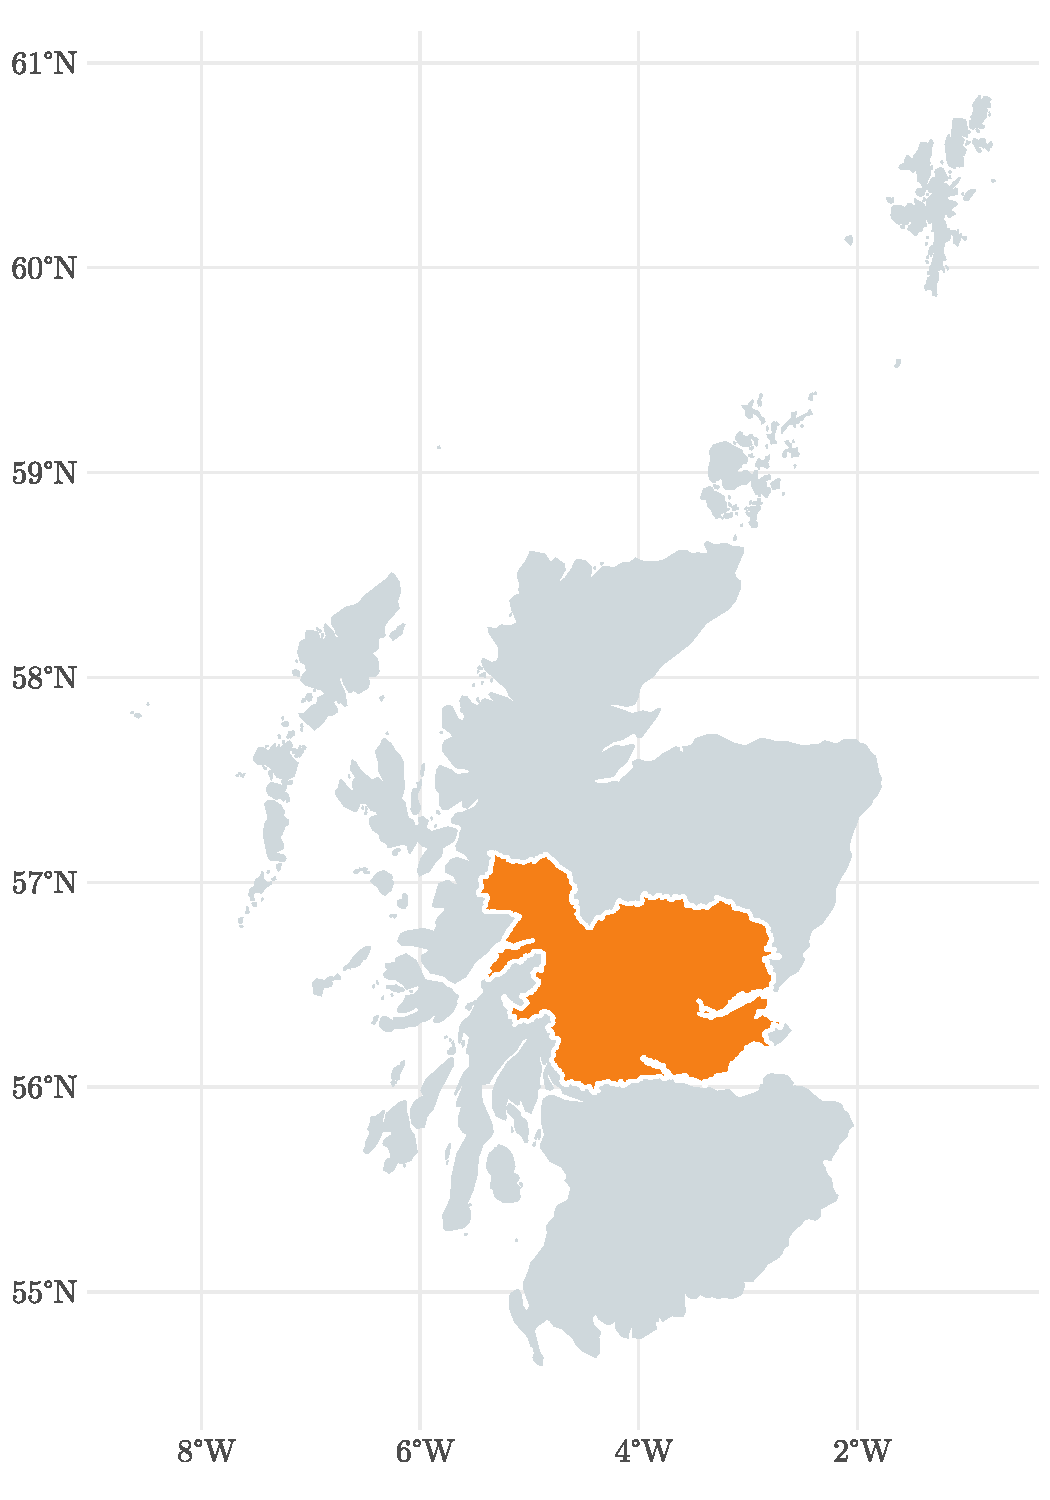
\includegraphics[width=0.4\linewidth]{output/figures/study_area.pdf}
    \label{fig:study-area}
    \caption*{\justifying \footnotesize Notes: Study region within Scotland (orange), capturing a buffer area around beaver expansion in the Tay, Earn, South Esk, Lunan, and Perth Coastal catchments. Agricultural parish boundaries are drawn in gray.}
\end{figure}

% % Data
% \section{Data}
% \label{sec:data}
% To estimate the impact of beaver reintroduction on agricultural land use, I obtain data on (1) the Tayside beaver expansion from three comprehensive regional surveys conducted over a decade, (2) high-resolution satellite-derived land use classifications, (3) soil data on agricultural land compatibility, (4) river level from a network of in-situ hydrometry monitors across Scotland, and (5) annual weather patterns. To measure the impacts of beaver entry on agriculture, I employ the land use data, exploiting its spatiotemporal variation, spanning pre- and post-beaver entry periods, to test for land use change. To detect physical environment changes following beaver entry, I use the hydrometry data. In robustness checks, I use high-resolution data on soil type, elevation, and slope to run models on subsamples varying beaver habitat suitability. In all analyses, the unit of observation is a 1km$^2$ cell in a grid constructed by tessellating the study region in Fig. \ref{fig:study-area}. Subsamples of only ``river'' cells rely on a watercourse layer sourced from Ordnance Survey OpenData (CITE?).

\subsection{Beaver Expansion}
Beavers reemerged in Scotland after 2000 around the River Tay, with anecdotal reports beginning around the middle of the decade and NatureScot, Scotland's national conservancy, acknowledging their presence in 2006. In 2012, NatureScot conducted the first comprehensive survey of beaver presence (\cite{campbell_rd_naturescot_2012}). Two follow-up surveys were conducted in 2017-18 and 2020-21, respectively, with each resurveying the extent of its predecessor as well as extensions along suitable habitat corridors. The surveys were carried out in canoe and on foot, with the 2012 survey covering 690km of contiguous watercourse and 450km of non-contiguous river bank around the rivers Tay, Tummel, Isla, Almond, and Earn.\footnote{An additional 310 km of river bank had been surveyed over several preceding years, informing the initial targets of the 2012 survey.} The 2020-21 survey covered 1,760km of contiguous watercourse, 1,238 non-contiguous spot checks along river banks (\cite{campbell-palmer_r_naturescot_2021}). Of the 1,522 field signs recorded in 2012, most were cutting, with only six direct beaver sightings. 98\% of field signs were found within 10m of a watercourse. I obtain beaver survey records via the National Biodiversity Network Trust's NBN Atlas repository, which contains a limited number of the variables recorded by surveyors. In data aggregation, I focus solely on the extensive margin of beaver expansion for several reasons. First, data sharing privacy constraints did not allow for collection of the full set of variables needed to estimate beaver population.\footnote{These include activity type (e.g., dam, foraging, scent mound), estimated age, distance from water, effected area, and river width/depth, among others.} Second, a change in GPS data collection methods in the 2017-18 survey inflated the number of observations linked to any given field sign, a discrepancy for which the full set of variables would be needed to adjust (\cite{campbell-palmer_r_naturescot_2018}). Finally, because much of the survey work was conducted during summer months, vegetation cover obscured many beaver signs, making precise quantification unreliable.

Over the decade of surveys, beaver populations expanded rapidly, more than doubling between each survey despite both official and unauthorized control operations. The 2012 survey detected 39 beaver groups in the Tayside region. In 2018, this had risen to 114 groups. In 2021, 251 groups were found (\cite{campbell-palmer_r_naturescot_2021}). Fig. \ref{fig:beaver-expansion} shows beaver expansion throughout the tessellated study region. Grid cells are colored according to the first year in which a NatureScot survey detected any beaver sign. The observed pattern accords with ecological literature on beaver colonization. Dispersal occurs linearly along waterways, both downstream and upstream (\cite{muller-schwarze_beaver_2011}), with separate groups initially far apart to avoid territorial conflict, then slowly filling over time (\cite{hartman_patterns_1995}).

\begin{figure}
    \centering
    \caption{Beaver Expansion}
    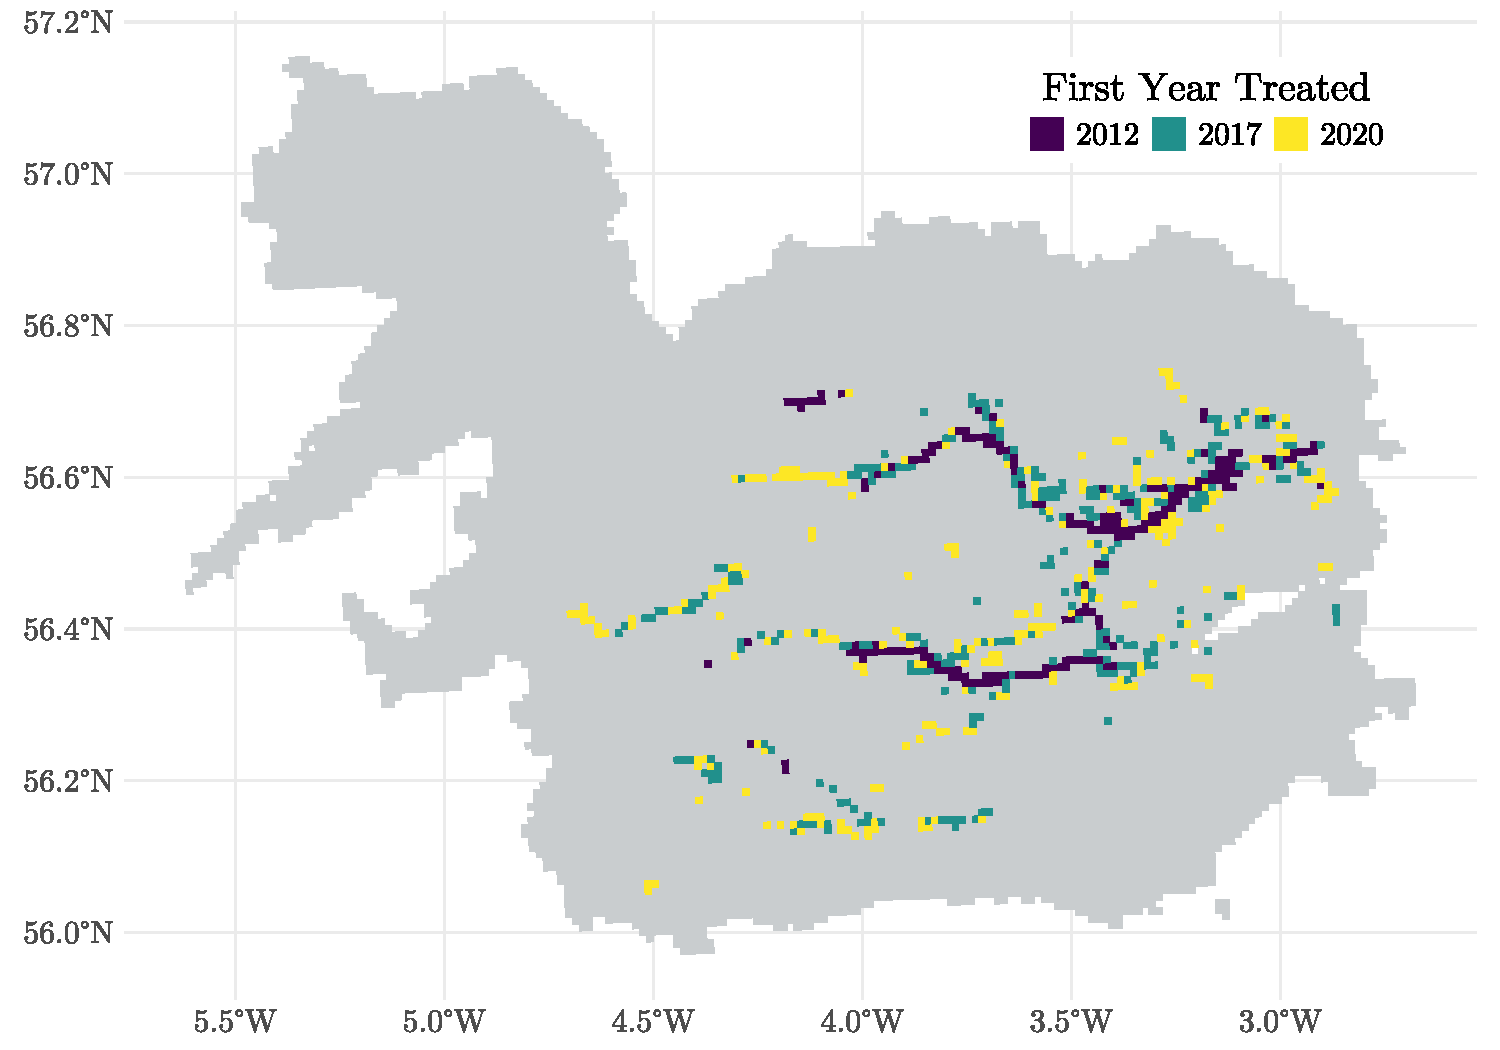
\includegraphics[width=0.7\linewidth]{output/figures/beaver_first_year_treated.pdf}
    \label{fig:beaver-expansion}
    \caption*{\justifying \footnotesize Notes: Beaver detection by survey year in study region. Observation units are 1km$^2$ landscape grid cells. Data source: NatureScot and affiliated survey contractors. See main text for details.}
\end{figure}

\subsection{Land Use}
To capture spatiotemporal variation in agricultural land use, I employ the UK Center for Ecology \& Hydrology's repeated Land Cover Map product (LCM) at 25m resolution, which exists for 1990, 2000, 2007, 2015, 2017, 2018, 2019, 2020, 2021, and 2022. The LCM covers the entirety of Great Britain and North Ireland, deriving its classifications from Sentinel-2 10-band seasonal composite image patches\footnote{Sentinel-2 was launched in 2015. 1990-2015 maps used Landsat 30m resolution imagery. In 2017, UKCEH revised its historical classifications to allow for comparability with post-2015 products.}, with additional context layers on height, aspect, slope, distance to built structures and water bodies, foreshore, and woodland to ejudicate spectral confusion \citep{noauthor_ukceh_2024}. Modern UKCEH models (since 2015) classify 10m pixels into 21 land use classes, based on the Biodiversity Action Plan Broad Habitats \citep{jackson_guidance_2000}, using a random forest. As ground truth, UKCEH uses pixels classified in previous years with high accuracy (>80\%) and no observed change over three consecutive years. Predictions made on 10m pixels are then aggregated to land parcels and from there rasterized at 25m resolution. I consider agricultural any pixel classified as ``arable'' in the UKCEH LCM, which includes cropped and freshly ploughed land (Fig. \ref{fig:ukceh-lcm-raw}). I do not include the closely related class of ``improved grassland'' due to its low recall and precision (74.3\% and 91.1\%, respectively) compared to ``arable,'' which has the highest recall and second highest precision of any class (97.6\% and 92.7\%, respectively), when validated on a set of reference points sourced from countryside surveys, National Forest Inventory, Rural Payment Agency, manual Sentinel-2 image interpretation, and UKCEH field collection.\footnote{This is largely due to the difficulty of differentiating between grassland types, including improved, neutral, calcareous, and acid, which exist on a spectral continuum.} Nearly all false negative arable pixels were mislabeled as improved grassland (93.4\%). Similarly, the majority of false positive arable-classified pixels were in fact improved grassland (55.8\%). I aggregate the 25m ``arable'' mask up to the 1km$^2$ grid cells to produce a measure on the unit interval of agricultural land share, weighting by overlap proportion for raster cells not entirely contained within the 1km$^2$ landscape cell (Fig. \ref{fig:ukceh-lcm-agg}). 

\begin{figure}
    \centering
    \caption{Agricultural land use}
    \begin{subfigure}{0.49\linewidth}
        \caption{\centering Agricultural land in 25m raster}
        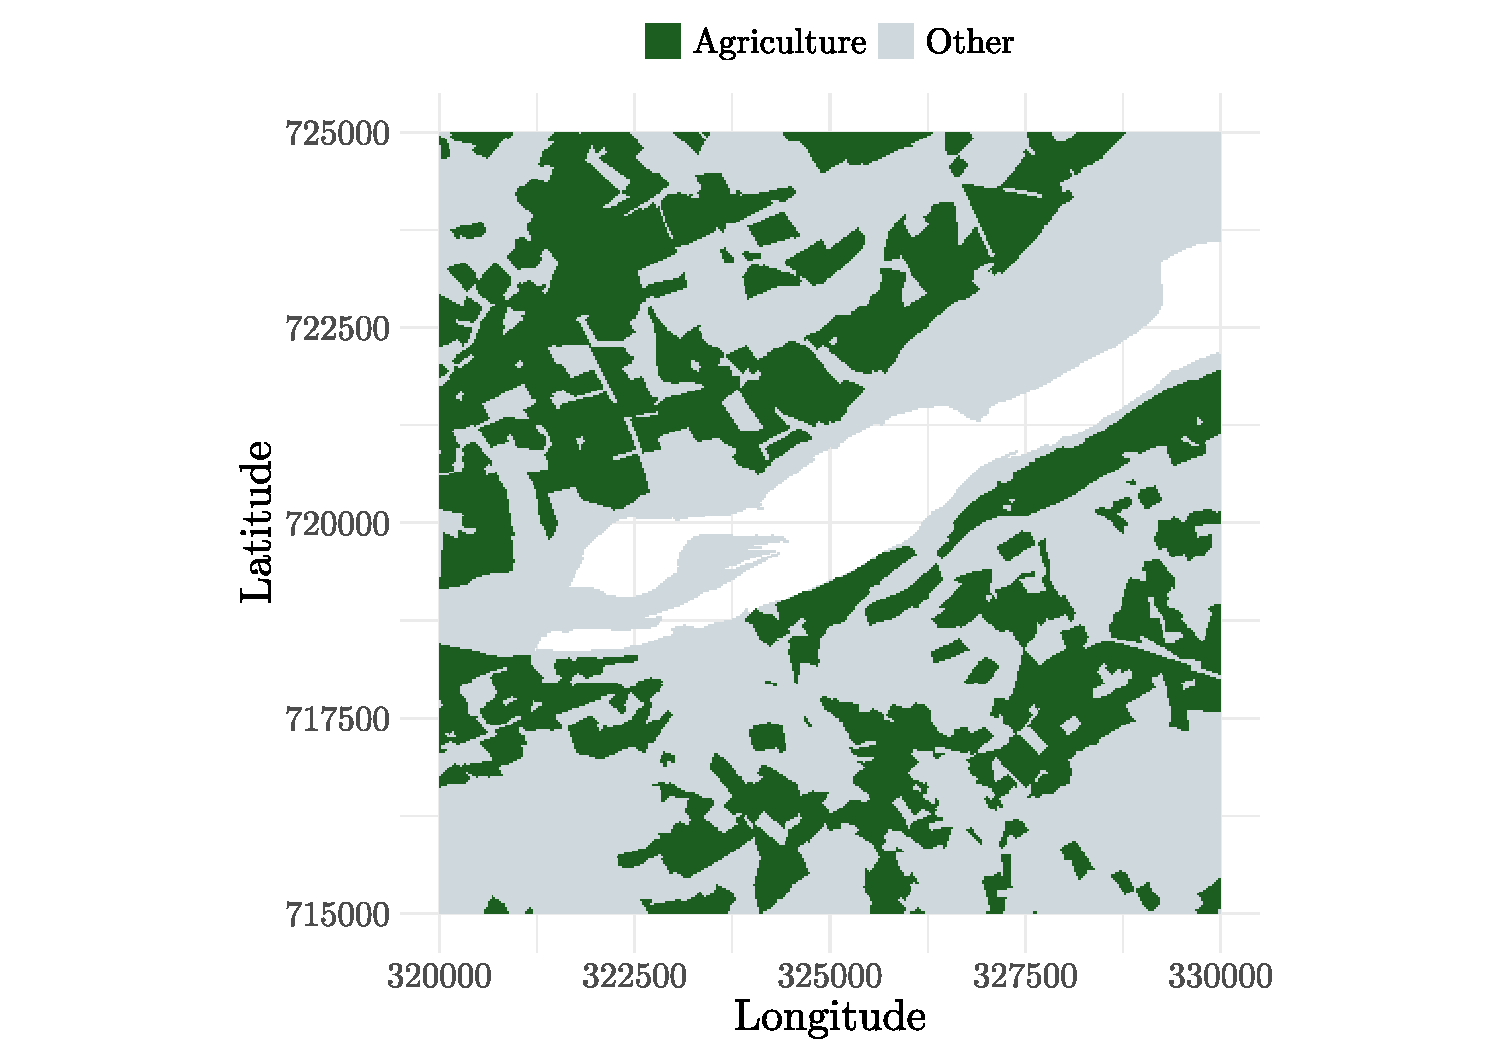
\includegraphics[width=\linewidth]{output/figures/lcm_example_area.pdf}
        \label{fig:ukceh-lcm-raw}    
    \end{subfigure}
    \begin{subfigure}{0.49\linewidth}
        \caption{\centering Agricultural raster aggregated to 1km$^2$ landscape grid cells}    
        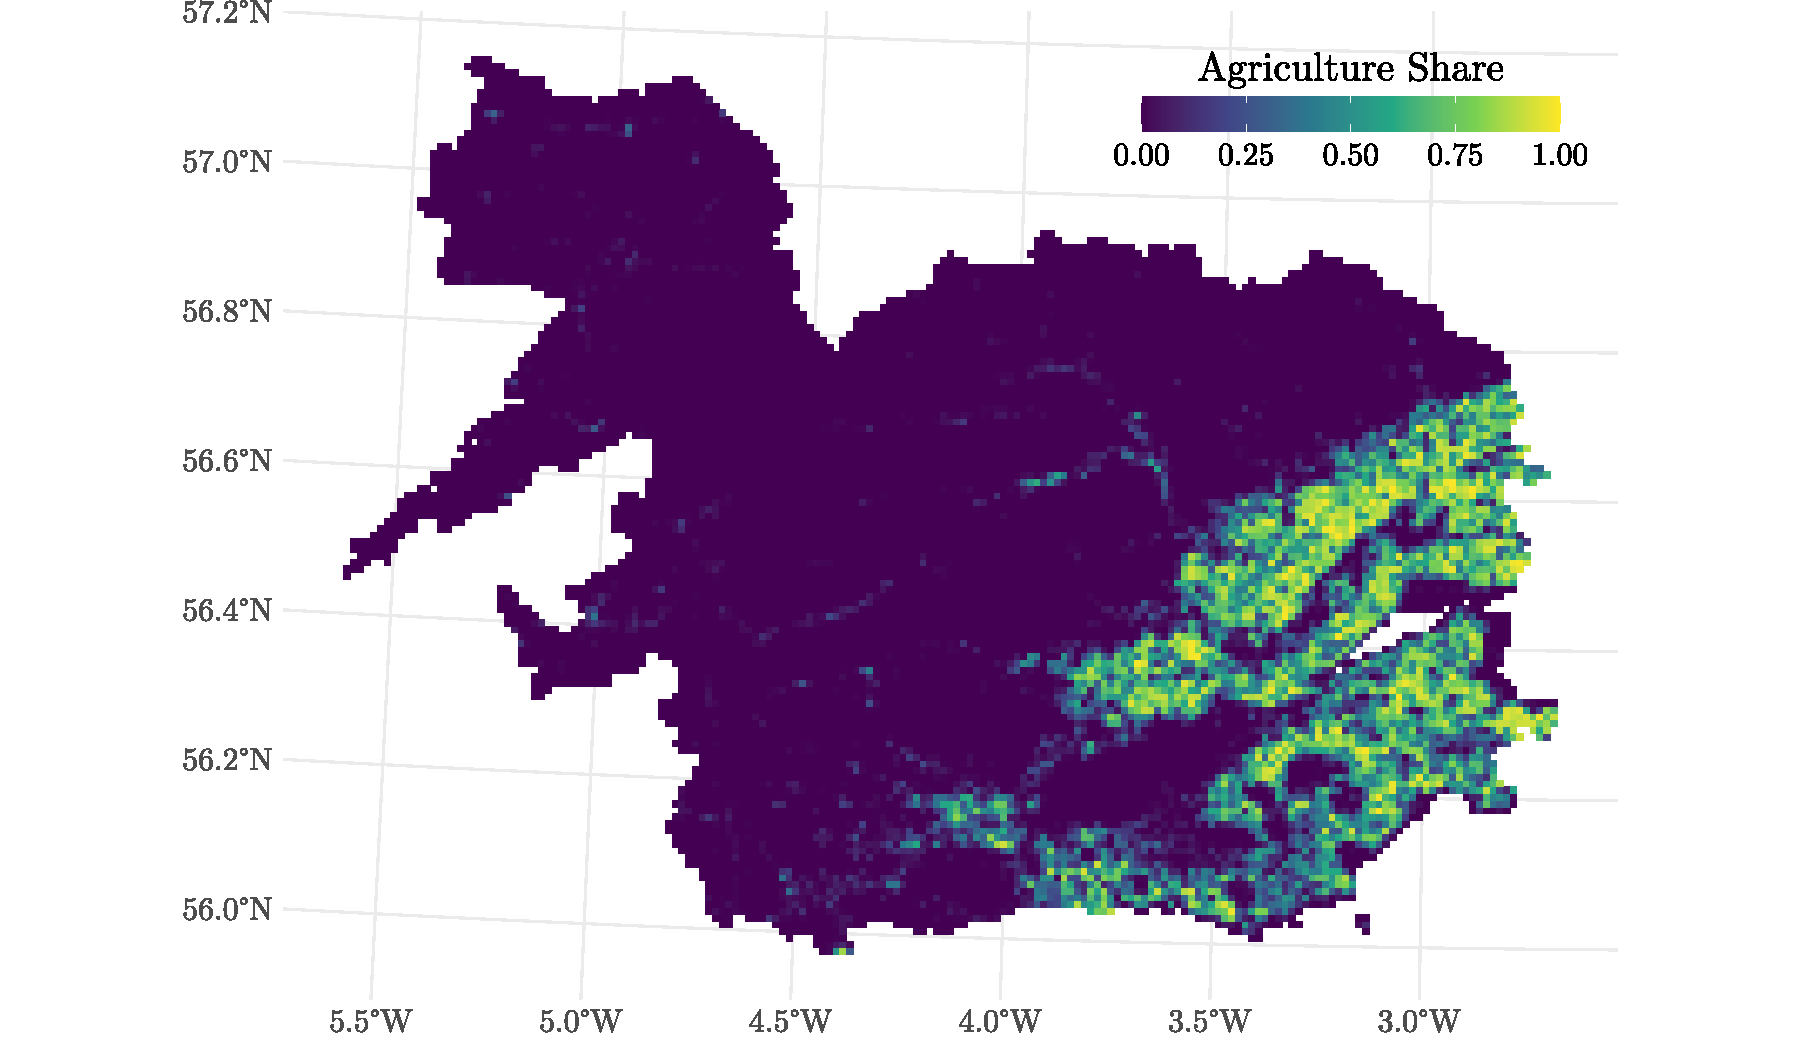
\includegraphics[width=\linewidth]{output/figures/lcm_agg_river_grid.pdf}
        \label{fig:ukceh-lcm-agg}
    \end{subfigure}
    \caption*{\justifying \footnotesize Notes: Data from the UK Center for Ecology \& Hydrology Land Cover Map (25m rasterized land parcels, GB). Fig. \ref{fig:ukceh-lcm-raw} shows the extracted agricultural layer in a subregion around the Firth of Tay. Fig. \ref{fig:ukceh-lcm-agg} includes the entire study region. 2022 data is used for illustration. See main text for details.}
\end{figure}

\subsection{Hydrometry}
To detect beaver impacts on their immediate surrounding, I obtain data on river characteristics. The Scottish Environmental Protection Agency (SEPA) operates a nationwide network of in-situ hydrometry monitoring stations, 167 of which reside in the study region. Stations collect data on rainfall, groundwater levels, river levels, river flow (or discharge), and tidal level. I extract historical records of river level, groundwater level, and river flow--all of which may be altered by beaver colonization. I drop groundwater level from analysis due to high missingness. I aggregate river level (recorded monthly) and river flow (recorded daily) to annual statistics to match the temporal resolution of the beaver expansion data.

\subsection{Soil}

% \begin{itemize}
%     \item Elevation from ASTER (https://lpdaac.usgs.gov/products/astgtmv003/). Slope calculated as first derivative of elevation (constant)
% \end{itemize}

To distinguish between high and low agriculture-propensity areas, I use soil data from the James Hutton Institute. The soil map bins Scottish land into 13 main soil classes, ranging from soil suitable for a broad array of crops\footnote{This highest cropping suitability category is characterized by ``well-drained deep loam, sandy loams, silty loams or their related humic variants with good reserves of moisture. Sites are level or gently sloping and the climate is favourable. There are no or only very minor physical limitations affecting agricultural use'' (cite)} to soil that could be used only for rough grazing (e.g., rugged or extremely wet terrain). An additional three classes capture built, water, and unmapped island areas. I group the 13 bins into three broad classes: Arable Cropping, Improved Grassland and Rough Grazings, and Non-Agricultural (including built, water, and unmapped areas). To achieve full cover, I employ two versions of the soil map: a 1:50,000 scale map that is considered definitive where coverage exists (mainly in eastern lowlands, where arable land is widespread) and a 1:250,000 scale map that provides lower resolution coverage in highlands areas not mapped by the 50k scale map. I calculate the share of each landscape grid cell that is occupied by a given class and determine the dominant class (>50\%) in each cell.

\subsection{Weather}

To control for variation in weather patterns across the study region, I extract temperature, precipitation, and vegetation cover records from the European Centre for Medium-Range Weather Forecasts' Reanalysis v5 (ERA5), a weather reanalysis product that provides hourly estimates at the resolution of a 31km global grid, spanning 1950 to present \citep{hersbach_era5_2020}. Using data from 1990 to 2022, I calculate annual total precipitation, average temperature at two meters, and average leaf area index. I then assign ERA5 annual grid cell values to 1km$^2$ landscape grid cells intersecting the ERA5 cell, weighting by overlap proportion when multiple ERA5 cells intersect with a single landscape cell.

% \subsection{Remote Sensing of Floods}

% % Zero Stage: Food emergencies and locust swarms 
% \section{Stage Zero}
% \label{sec:stage_zero}
% \input{sections/stage_zero_food_security.tex}

% % Empirical Strategy 
% \section{Methods}
% \label{sec:methods}
% I estimate response functions to beavers of both local environmental characteristics (namely, stream level and flow intensity) and land used for agriculture.

\subsection{Environmental Response to Beaver Entry}

Using [n] number of landscape grid cells in which I observe beaver entry, I estimate the classic two-period difference-in-difference model

\begin{equation} \label{eq:did_main}
y_{it} = \alpha_i + \gamma_t + \beta^{b}D_{it} + \mathbf{X}_{it} + \epsilon_{it},
\end{equation}

where $y_{it}$ are the environmental outcomes (stream level and flow), $\beta^b$ is the effect of being treated by beaver presence, $D_{it}$ captures beaver treatment, $\mathbf{X}_{it}$ is a vector of time varying local environmental characteristics, and $\epsilon$ is a random error term. $\alpha_i$ and $\gamma_t$ capture grid cell and pre-and post-period fixed effects, respectively.



\subsection{Land Use Change}

Using the model specified in \eqref{eq:did_main}, I estimate the impacts of beaver entry on the proportion of land area in a grid cell that is in agricultural use. 

% % Results 
% \section{Results}
% \label{sec:results}
% 
Preferred specification of beaver impacts on agricultural land share, river level, and river flow.

\begin{table}[htbp]
   \caption{Beaver impacts on agriculture and river characteristics.}
   %\bigskip
   \centering
   \begin{tabular}{lcccc}
      \tabularnewline\midrule\midrule
                                    & Share Agri.   & River level (mean) & River level (max) & River flow (mean)\\  
                                    & (1)           & (2)                & (3)               & (4)\\  
      \midrule 
      Beaver Presence               & 0.017$^{***}$ & -0.034             & 0.063             & -0.054\\   
                                    & (0.005)       & (0.026)            & (0.076)           & (0.269)\\
      \midrule
      Observations                  & 28,388        & 157                & 157               & 119\\  
      Within R$^2$                  & 0.002         & 0.027              & 0.010             & 0.001\\  
      Mean Dep Var                  & 0.125         & 0.843              & 2.467             & 16.400\\  
       \midrule
      Landscape cells fixed effects & $\checkmark$  & $\checkmark$       & $\checkmark$      & $\checkmark$\\   
      Period fixed effects          & $\checkmark$  & $\checkmark$       & $\checkmark$      & $\checkmark$\\   
      \midrule \midrule & \tabularnewline
   \end{tabular}
   \justifying \footnotesize
   Each column reports results from a two-way fixed effects regression.   Landscape grid cell and time period (pre- and post-beaver entry) are included.   Standard errors are clustered at the landscape grid cell level.   Regression sample includes all never-treated and ever-treated units.
\end{table}


% \section{Discussion}
% \label{sec:discussion}
% \input{sections/discussion.tex}


\printbibliography

% Appendices 
\setcounter{page}{1}
\setcounter{table}{0}
\setcounter{figure}{0}
\setcounter{section}{0}
\renewcommand{\thetable}{\thesection\arabic{table}}
\renewcommand{\thefigure}{\thesection\arabic{figure}}
\renewcommand{\thepage}{\thesection\arabic{page}}
\renewcommand\thesection{\Alph{section}}
\renewcommand\thesubsection{\thesection.\arabic{subsection}}
\newpage
\section*{Appendix}
\section{Additional Results}
\input{appendix/additional_results.tex}

\setcounter{page}{1}
\setcounter{table}{0}
\setcounter{figure}{0}
\renewcommand{\thetable}{\thesection\arabic{table}}
\renewcommand{\thefigure}{\thesection\arabic{figure}}
\renewcommand{\thepage}{\thesection\arabic{page}}
\renewcommand\thesection{\Alph{section}}
\renewcommand\thesubsection{\thesection.\arabic{subsection}}
\newpage
\section{Data Construction}
\input{appendix/additional_data.tex} 


\begin{comment}
\setcounter{page}{1}
\setcounter{table}{0}
\setcounter{figure}{0}
\renewcommand{\thetable}{\thesection\arabic{table}}
\renewcommand{\thefigure}{\thesection\arabic{figure}}
\renewcommand{\thepage}{\thesection\arabic{page}}
\renewcommand\thesection{\Alph{section}}
\renewcommand\thesubsection{\thesection.\arabic{subsection}}
\newpage
\section{Supplementary Background on Locusts' Biology}
\input{appendix/additional_background}
\end{comment}

\end{document}
